\documentclass[titlepage,a4paper,12pt,]{article}
\usepackage{graphicx} % Required for inserting images
\usepackage{float}
\usepackage{setspace}
\usepackage{url}
%\usepackage{minted}
\usepackage{booktabs}
\usepackage{geometry}
\usepackage{parskip}
\usepackage{ragged2e}
\usepackage{subfig}
\usepackage{cite}
\usepackage[svgnames]{xcolor}
\usepackage{makecell, tabularx}
    \setcellgapes{2pt}
    \makeatletter
    \newcommand*{\compress}{\@minipagetrue}
    \makeatother
    \newcolumntype{I}{ >{\RaggedRight\compress\itemize}X<{\enditemize}}
    \newcommand*{\mcl}[1]{\multicolumn{1}{l|}{#1}}
\usepackage[skip=1ex]{caption}
\usepackage{enumitem}\usepackage{tabularx}
\usepackage[utf8]{inputenc}
\usepackage[T1]{fontenc}
\graphicspath{ {./pictures/} }
\onehalfspacing

\begin{document}

\begin{titlepage}
\begin{center}
  \bfseries
  \huge UNIVERSITY OF SOUTHERN DENMARK
  \vskip.1in
  \textsc{\LARGE Faculty of engineering}
  \vskip.1in
  \large BEng Mechatronics
  \vskip.1in
  \Large Mechatronics Semester Project 4
  \vskip0.1in
  \emph{\huge Ladybug}
\end{center}

\vskip0.7in

\begin{minipage}[10pt]{.18\textwidth}
  \begin{flushleft}
    \bfseries\large Supervisor:\par \emph{Lars Duggen} \par \emph{Davi Goncalves Accioli} \end{flushleft}
\end{minipage}
\hskip.4\textwidth
\begin{minipage}{.4\textwidth}
  \begin{flushleft}
    \bfseries\large Group: 7 \par \emph{Tobias Blaabjerg Karlsen} \par \emph{Artis Fils} \par \emph{Thor Uerkvitz} \par \emph{Choyon Mainul Hasan} \par \emph{Johan Paul} \par \emph{Ruta Miglava}
  \end{flushleft}
\end{minipage}

\vfill
\centering
\bfseries
\Large Year \the\year
\end{titlepage}


\section{Background}

The ability to fly has always been very desirable. The first unmanned aircrafts can be dated back to 1849 when Austria utilised unmanned air balloons filled with explosives to attack Venice. \cite{Vyas2020}
Ever since then unmanned aircraft vehicles (UAV) have experienced vast tehnological development and are defined as machines controlled by means of pre-programmed flight control, as defined by the ECAA Transport Agency \cite{Droner}, nowadays called drones, have risen in popularity.

Because of this, UAVs come in a wide range of sizes and weights.
UAVs often include multirotors, radio-controlled miniature helicopters, and aeroplanes \cite{Ann2012}.
As a result, there are several methods to categorize drones. The performance parameters of UAVs, such as weight, wingspan, wing load, flight range, maximum flying altitude, speed, and production cost, are typically used to categorize them \cite{Hassanalian2017}.
Depending on how the lift is produced, drones may also be divided into fixed-wing and rotating-wing types.
According to the drone code categories, the European Aviation Safety Agency (EASA) categorizes unmanned aircraft by weight.
The EASA regulations for open categories (drones without an EASA class designation), are summarized in a simple overview in Figure~\ref{fig:Table} \cite{Euasa}.

Self-built drones weighing up to 250 grams, as described in Figure~\ref{fig:Table}, may be used without registration if the drone is a toy or the drone is not equipped with a camera. All other drones must be registered and the pilot must pass examinations \cite{Euasa}. In this paper, self-built rotary drones with four wings or propellers are the objective, making weight-based classification suitable.

\begin{figure}[H]
    \centering
    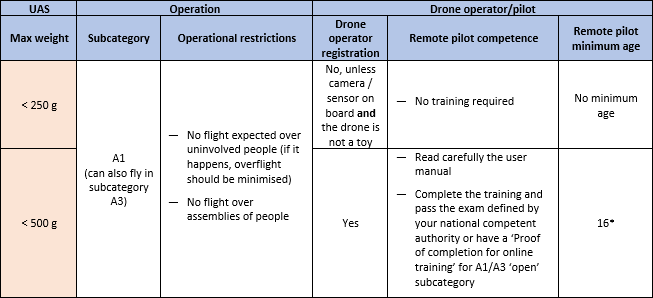
\includegraphics[scale = 0.9]{pictures/classification.PNG}
    \caption{Classification and restrictions for non-EASA class drones \cite{Euasa}}
    \label{fig:Table}
\end{figure}


When it comes to the state-of-the-art project, PULP-DroNet is a deep learning-powered visual navigation engine that enables autonomous navigation of a pocket-size quadrotor in a previously unseen environment. Thanks to PULP-DroNet the nano-drone can explore the environment, avoiding collisions even with dynamic obstacles, completely autonomously -- with no human operator and no ad-hoc external signals. This means that all the complex computations are done directly aboard the vehicle and very quickly. The visual navigation engine is composed of both a software and a hardware part. \cite{Niculescu2021}

When it comes to the future, the simulated pollination of agricultural plants by means of nano-copters could provide collecting and delivering pollen by means of autonomous control. A design of nano-copter for pollination can be made on the basis of innovative modifications of existing models by reprogramming flight controller that is to be fully adapted to computer interface. The robotic system is offered specially for artificial pollination in conditions of greenhouses and minor agricultural enterprises. \cite{Abutalipov2016}

\section{Problem statement}

The utility of smaller drones are immense, where it can be used in surveillance, toys and potentially to also be part of a swarm of drones. Although, there are smaller drones existing in the current market, we would like to challenge ourselves to build one ourselves, where certain goals ranging from functionality to budget are listed below.


\subsection{Primary goals }
\begin{itemize}
    \item
          Net maximum weight of the drone is 250 grams. Weight under 250 grams ensures it falls under A1 category in EU regulations. 1
    \item
          Flight time of 20 seconds.
    \item
          Stress of the structural system should not exceed rupture point. System does not experience fracture.
\end{itemize}


\subsection{Secondary goals}
\begin{itemize}
    \item
          Flight time of minimum one minute.
    \item
          Can land with acceleration less than 9.8 m/s2.
    \item
          Stress of the drone system should not exceed the yield point. System does not experience plastic deformation.
    \item
          Drone is remote controllable.
    \item
          Drone can fly in formation with another identical drone.
    \item
          Total production cost of the drone is under 500 DKK (Not including remote controller).
    \item
          Drone can play audio.
\end{itemize}



\subsection{Constraints}

\begin{itemize}
    \item
          Budget for entirety of project is 2000 DKK.
    \item
          Time available to finish the project is 4 months.
    \item
          Drone should have a minimum hover time of 5 seconds.
    \item
          Drone should be fully functional and able to take off again after landing.
    \item
          No use of flight controller software or unmanned vehicle Autopilot software Suite, capable of controlling autonomous vehicles.
\end{itemize}


\section {Test Specifications}
\subsection{Primary goals:}
\begin{itemize}
    \item
          To test this, the drone will be weighed with a scale of a precision on 0,1 grams.
    \item
          In order to test the flight time, a stopwatch will be started from the moment the drone leaves the ground and is stopped as soon as it lands.
    \item
          This goal will be the tested trough FEM, ensuring that the chosen material for the drones body, will not rupture.
\end{itemize}

\subsection{Secondary goals}
\begin{itemize}
    \item
          This will be tested with the same method as primary goals tests point 2.
    \item
          This will be tested with a mobile phone, recording the drones landing, using the drones position compared to the timestamp of the video.
    \item
          This will be tested with the same goals as primary goals test point 3.
    \item
          This will be tested by the possibility of sending wireless signals to the drone, with the drone reacting to those send signals.
    \item
          This will be tested purely by ear, listening to the drones output.
    \item
          This will be tested by mobile phone video, looking at the drones positions at given timestamps.
    \item
          This will be tested trough summing the price for each single part, ensuring that it doesn’t exceed 500 DKK.
\end{itemize}

\subsection{Constraints}
\begin{itemize}
    \item
          This will be done with the same method as the secondary goals test, though ensuring the project cost is over 2000 DKK.
    \item
          To evaluate the time constraint point of the project, the goal fullfilments will be evaluated in the end of the project period. In the case that all primary goals are fulfilled, the constraint is succeeded.
    \item
          This will be tested with a stopwatch, ensuring that the hover time is atleast 5 seconds.
    \item
          This will be tested with making the drone take off right after a landing, making sure that the drone is fully operational at the second take-off.
    \item
          This will fulfilled by not employing any of the aforementioned in the drone.
\end{itemize}
\subsection{Risk Assesment}

To ensure the safety under operation and development of the drone, a risk assessment is created for the drone project, based on the Fine \& Kinney method \cite{finekinney}.

\begin{figure}[H]
    \begin{center}
    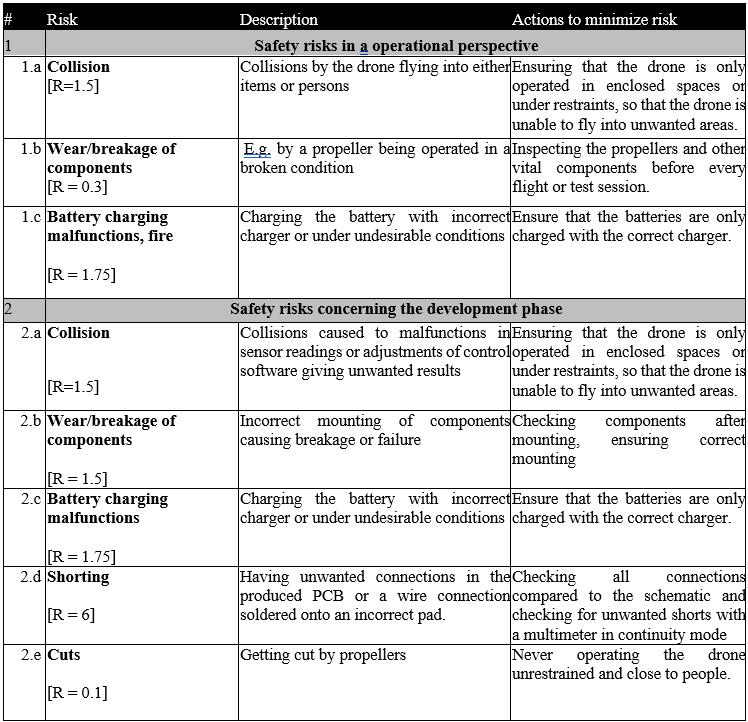
\includegraphics[scale=0.7]{pictures/Risk assesment table.png}
    \end{center}
    \caption{Risk assesment table}
    \label{Risk assesment table}
\end{figure}

Marked in all the risks are the risk scores calculated by the Fine \& Kinney method of Risk, Risk score = Probability * Exposure * Consequence. These risk scores are then compared in the risk clusters of the method, with five defined classes. After calculating the proposed risk ratings of the found risks, it’s apparent that all risks fall under the lowest factor of the Fine \& Kinney method of scores the: ‘Risk; Perhabs acceptable category’. 


\subsection{GitHub Interaction}
Each semester project has a main focus-point for educational purposes. The main focus-point for SPRO4 is control engineering which covers implementations such as IMU combined with programming and PID for the drone. This means a lot of the project development will be software related.

Working together in a large group for a single deterministic purpose can be cumbersome, so in order to better track progress, a GitHub repository has been made to share files and collaborate more effectively. GitHub requires little to no extra effort to implement and use, and will only require a small change in work culture to use correctly, potentially saving a lot of time.

 The GitHub repository is an easy way to share and keep track of the software development progress, and gives many advantages when working with embedded systems. 

\subsubsection{Advantages of Using GitHub}
- GitHub works by having one main code or branch which is shared between everyone. Users can then create their own branches and work on something individually, before it is sent back to the main. This means past revisions of work can be saved and reviewed by everyone, and changes can easily be reverted if a fundamental mistake occurs - or is spotted during development. Mistakes in the software are also easier to identify and can be solved without having to change the main program at all. This also means that changes can be made without interfering with other peoples' workflow, giving a clear advantage when working/collaborating on similar problems in the software.\cite{benefitsGithub}
With GitHub, open source software becomes easily available and secure, while also being compatible with other GitHub repositories. This means GitHub can also be used to keep dependencies up to date for already existing projects, and provide live updates to multiple libraries and dependencies automatically and safely. \cite{githubaccelerates}

\subsubsection{Usefulness Beyond the Project}
GitHub is very standard among many engineering companies, and is one of the most widespread UML service. It is used by many companies in the industry, so it's very useful to familiarize with GitHub before entering jobs-market, especially in software development.
And with GitHub's wide usage and accessibility it has quickly become the world's largest software collaboration tool in the world with over 100 million developers.\cite{WhoGithub} GitHub is also owned by Microsoft, and works with Microsoft programs, which is very standard for many work environments, providing high compatibility.

All in all, GitHub seems to be a necessary skill to have in the future as an engineer.


\section{Design and manufacturing of quadrotor} 

The main body of the drone is created as a PCB, in order for the body to host both the structural element and the electrical connections of the drone. Since the project formulation’s main goals dictates the drones size and mechanical properties, the drones size was chosen to be $100 mm^2$, so that the PCB could accommodate all the needed components of the drone. The PCB shape itself was designed in Siemens NX as a simple outline with holes for the motor mounts. This outline was exported in a DXF format into Autodesk Eagle were the actual PCB was designed from the needed electrical circuit. The electrical schematic was created in Eagle’s schematic designer and then automatically converted to a PCB board with the auto-router feature. The trace width of the PCB is specifically chosen to be 30 mills so it can supply the needed 1.72 amps \cite{PCBTracewidth} for the motors at maximum rpm. The microcontroller of the drone is mounted by pin headers, the motors by the motor mounts and the remaining components by soldering onto the top layer. The position of the microcontroller is offset from the center, in order to ensure that the In-built 6-axis IMU is centered to the exact middle of the PCB.

\begin{figure}[H]%
    \centering
    \subfloat[\centering CAD View]{{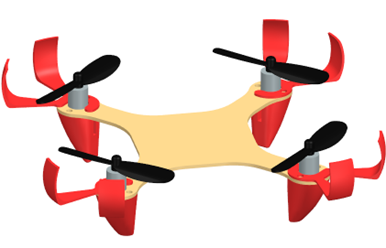
\includegraphics[width=5cm]{design/DroneCAD.png} }}%
    \qquad
    \subfloat[\centering PCB View]{{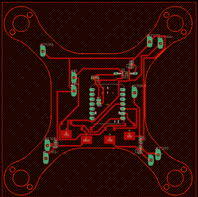
\includegraphics[width=5cm]{design/PCBpicture.png} }}%
    \caption{Drone model}%
    \label{fig:example}%
\end{figure}

In order to control the speed of the motors, one of the potential options would be to use an H-bridge to control
the DC motors. However that would be excessive, as the motors does not need to run in reverse as contain many components
As a less power consuning simple and lighter option, a single N-channel mosfet was used for each motor.

\begin{figure}[H]
    \begin{center}
    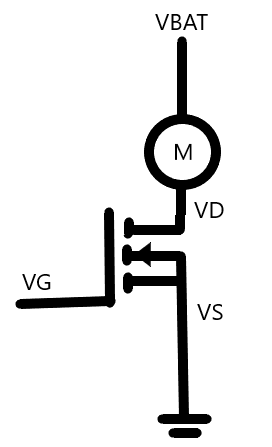
\includegraphics[scale=0.7]{design/Mosfet_Control}
    \end{center}
    \caption{Motor control with MOSFET.}
    \label{fig:Mosfet_Control}
\end{figure}

As illustrated in figure \ref{fig:Mosfet_Control}, the drain of the MOSFET is connected to the motor, which is supplied by 
the battery, and the source of the MOSFET is grounded. Meanwhile, the VG pins are connected to one of the PWM pins 
of the nRF52840 MCU, where the opening of the gate is proportional to the PWM. Thus, when VG (simulated by PWM) is 
smaller than the V threshold of the MOSFET, the motors are static, and if VG surpasses V threshold, then the motors 
start spinning with higher RPM as PWM is increased. 
The MOSFETs used for this situation are FDD8896 \cite{FDD8896}, as it has 
a low threshold voltage of 2.5V (MCU pins can supply 
up to 3.3V), and can handle up 94A in continuous drain 
current.

As there is high currents being drawn from the motors, one of the things needed to be configured was protection 
against overcurrent being drawn from the microcontroller. When the motors are switched on or off, 
a surge current arises which can result in additional overcurrent being pulled from the microcontroller if 
the battery is not alone capable of supplying the current. 

\begin{figure}[H]
    \begin{center}
    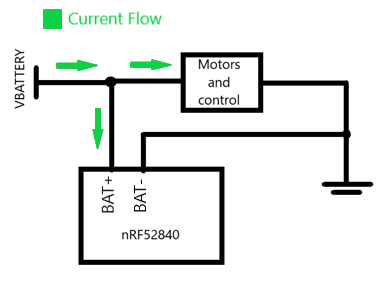
\includegraphics[scale=0.7]{design/Continuous_Current}
    \end{center}
    \caption{Current flow during continuous operation.}
    \label{fig:Continuous_Current}
\end{figure}

\begin{figure}[H]
    \begin{center}
    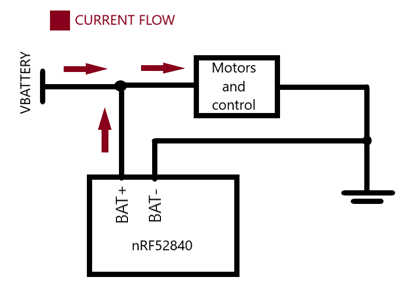
\includegraphics[scale=0.7]{design/Surge_Current}
    \end{center}
    \caption{Potential current flow due to surge current.}
    \label{fig:Surge_Current}
\end{figure}

In order to prevent reverse current from the MCU, 
during a surge, one of the potential options to utilise would be a diode placed in the following 
configuration. 

\begin{figure}[H]
    \begin{center}
    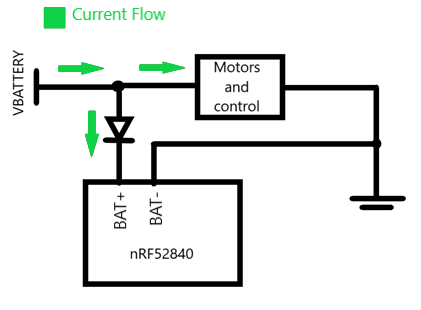
\includegraphics[scale=0.7]{design/Diode_Protection}
    \end{center}
    \caption{Diode added to prevent reverse current flow from MCU.}
    \label{fig:Diode_Protection}
\end{figure}

Additionally decoupling capacitors were added in 
parallel to the positive and negative motor pins 
and the MCU BAT+ and BAT- pins.

\begin{figure}[H]
    \begin{center}
    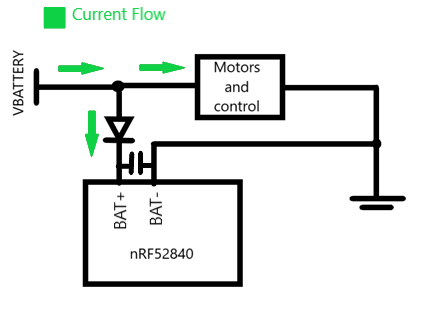
\includegraphics[scale=0.7]{design/Diode_Protection_&_decoupling_capacitors}
    \end{center}
    \caption{Example of decoupling capacitor for stable voltage to MCU.}
    \label{fig:Diode_Protection_&_decoupling_capacitors}
\end{figure}

The diode utilised is 1N5818 \cite{1N5818}, as it has a low 
forward voltage of under 0.5V, resulting in low 
power losses. Moreover, the decoupling capacitors
are cermaic capacitors as they generally smaller
in size, and they are rated at 100 nF, which follows 
the general guidelines of decoupling capacitor values.
\cite{DecouplingCap}

With the combination of the CAD-outline and the electrical schematic, PCB Gerber files could be output for production. The only excess parts needed for the drone would be motor mounts and prop guards (prop guards solely for testing, not for final use). The Motor mounts act as both landing legs and motor mounts. They would be designed in order for the motors to press fit into the central hole, mounted onto the PCB by screws into the motor mount going through the PCB. The designed mounting parts was printed in PLA on a Prusa MK3S+ 3D printer. The Parts were printed with a single perimeter and 3\% infill in order for each leg to weigh 1.1 grams while still having the nescessary structure to have a stable press-fit. 

\begin{figure}[H]%
    \centering
    \subfloat[\centering Motor Mount]{{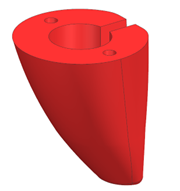
\includegraphics[width=3cm]{design/Droneleg.png} }}%
    \qquad
    \subfloat[\centering Mounted Motor]{{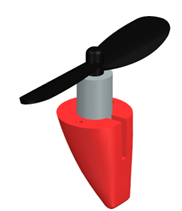
\includegraphics[width=3cm]{design/Dronepressfit.png} }}%
    \qquad
    \subfloat[\centering Prop Guard]{{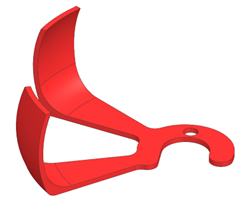
\includegraphics[width=3cm]{design/Dronepropguard.png} }}%
    \caption{3D-Printed drone parts}%
    \label{fig:example}%
\end{figure}

The project formulation states that the “Stress of the drone’s structural system should not exceed rupture point. System does not experience fracture”. This was tested through Ansys Mechanical Static Structural Analysis. Using the CAD model of the drone, the following boundary conditions were applied: Fixed constraint on the bottom area (excluding the drones arms), Z direction forces (upwards) was applied on each of the motor mount screw holes according to the found motor thrust, a single force vector in the Z direction (downwards) was applied to the top face (excluding the drones arms), to resemble the gravity force caused by the weight of the drone. Besides the boundary condition, the setup contained a mesh refinement of 3 steps, a material assignment of FR4 Fiber Glass Epoxy Board and a solution setting of equivalent stress. Below is a picture of the stress simulation of the initial design, which showed clear stress concentrations in the corners where the motor arms runs into the body section. The stress concentration had a magnitude of 1.6839 MPa which is satisfactory regarding the requirement of fracture, since the tensile strength of the given material is 320 MPa \cite{FR4}. 

\begin{figure}[H]%
    \centering
    \subfloat{{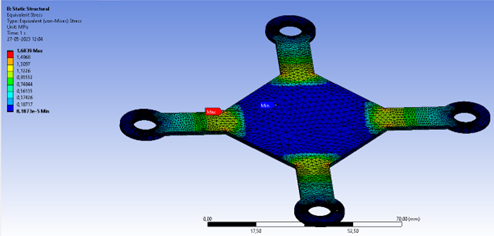
\includegraphics[width=10cm]{design/Ansys1.png} }}%
    \caption{Initial Ansys Simulation}%
    \label{fig:example}%
\end{figure}

Although it was clear that the drone body would be strong enough to operate under max power, the stress concentrations were undesirable. Therefore 20 mm radii was added to the stress all corner points of the drone body. Repeating the simulation with the same boundary conditions, it was clear that the added radii removed the stress concentrations and instead distributed the stress over a broader area of the motor arms. Furthermore, it was found that the maximum stress was found to be 0.87154 MPa, which is approximately half the maximum strength of the initial model that had the stress concentrations.

\begin{figure}[H]%
    \centering
    \subfloat{{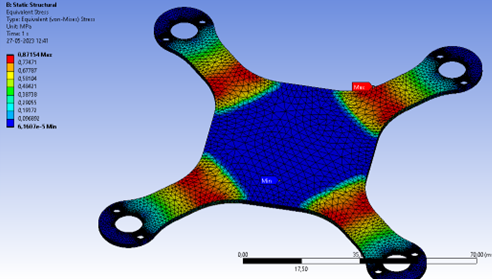
\includegraphics[width=10cm]{design/Ansys2.png} }}%
    \caption{Final Ansys Simulation}%
    \label{fig:example}%
\end{figure}

To power the drone a single cell Turnigy Li-Po battery is used, at 3.7 - 4.2 V and 300 mAh. The battery is chosen specifically to be able to supply the needed current of the drone. With a C-rating of 35C, the battery is able to discharge continously at 10.5 amps which is sufficent for the electrical circuit. The motors used are 8520 brushed Coreless DC-motors, which properties are characterized in the control chapter under thrust testing using the stock 2-bladed propellers that the motors were shipped with. 

\begin{figure}[H]%
    \centering
    \subfloat[\centering Turnigy Battery]{{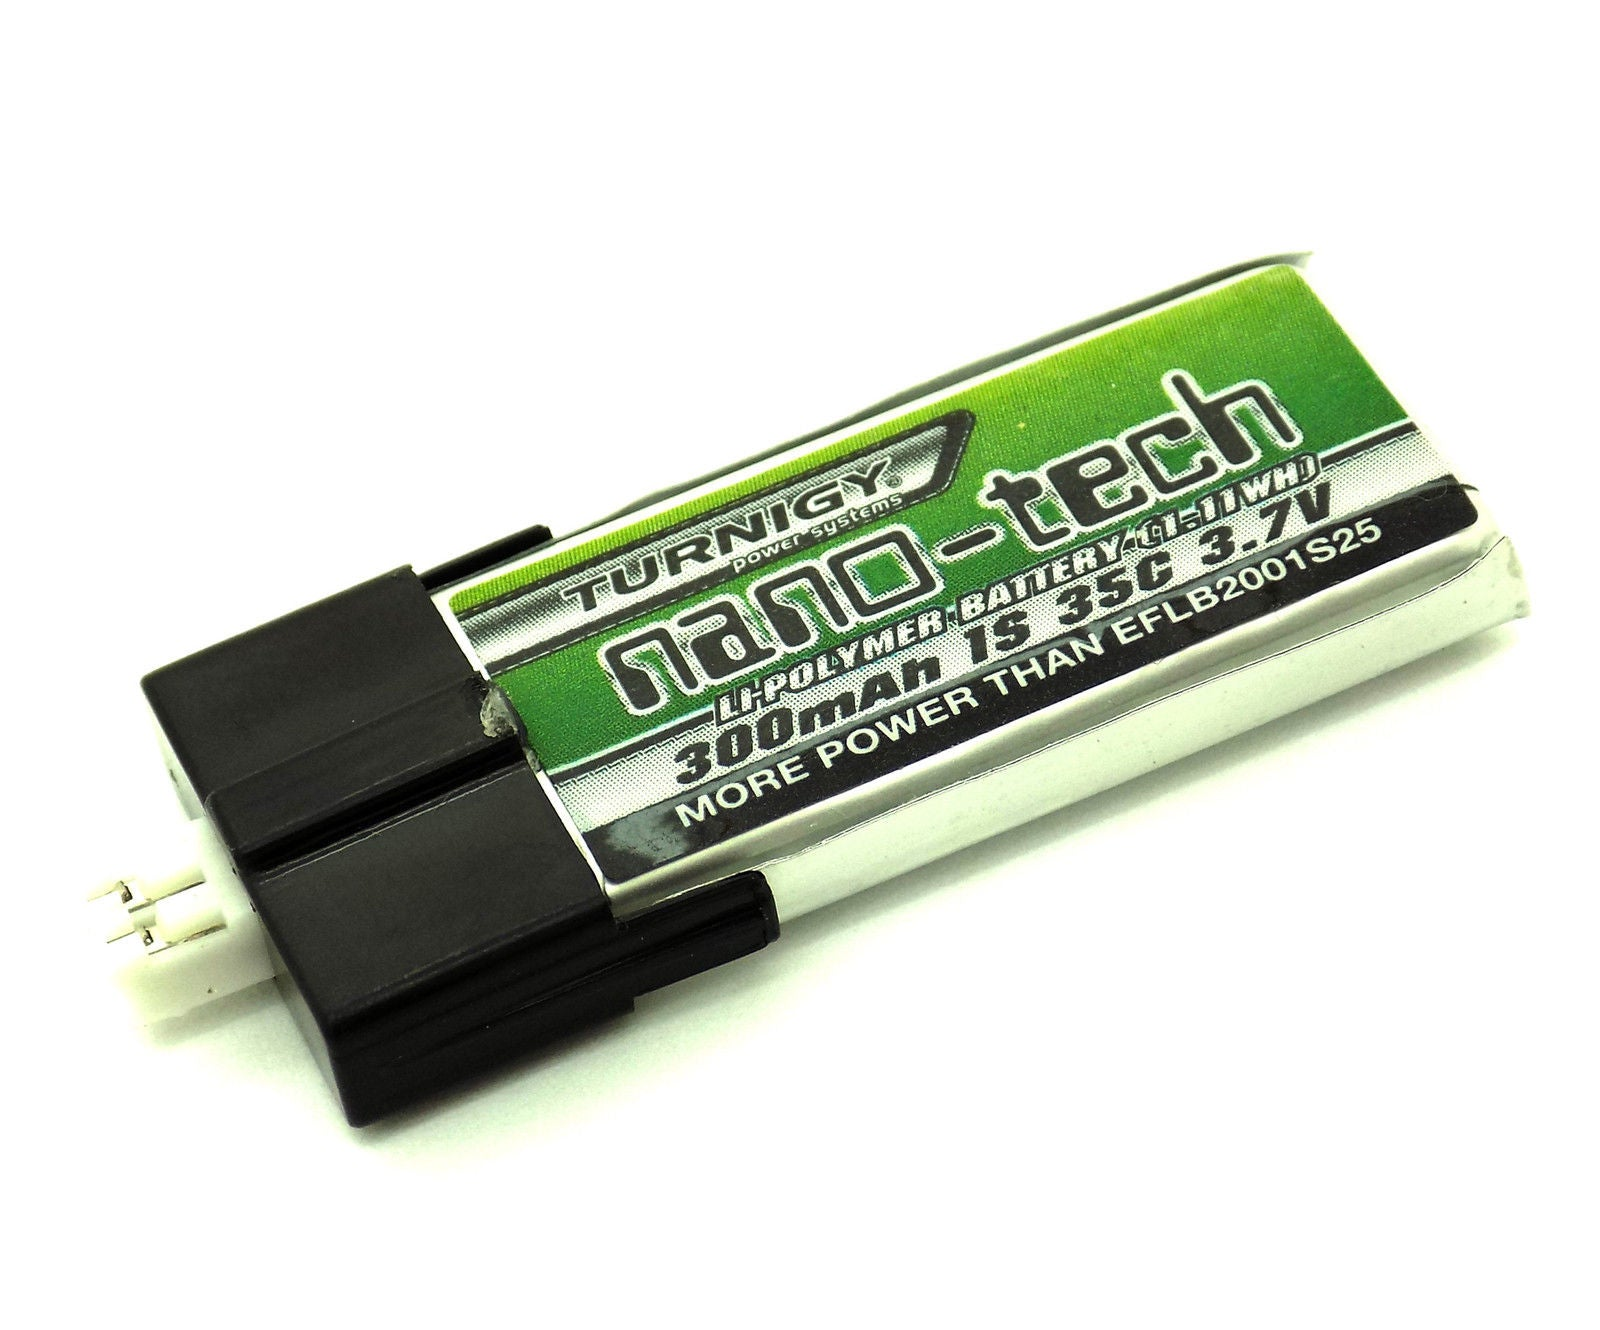
\includegraphics[width=5cm]{design/battery.jpeg} }}%
    \qquad
    \subfloat[\centering 8520 DC-motor]{{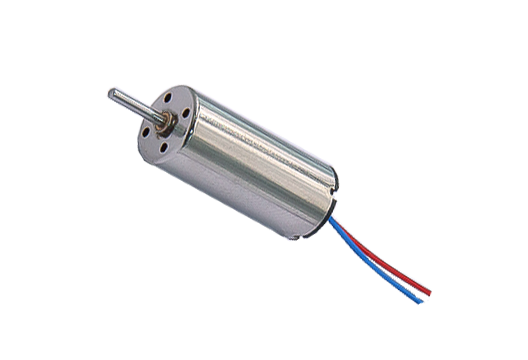
\includegraphics[width=5cm]{design/8520.jpg} }}%
    \caption{Motor and Battery used on the drone}%
    \label{fig:example}%
\end{figure}

After assembly of the drone including all the parts, it became apparent that the initial weight estimation of the drone was too low. After weighing the final physical setup it weighed 70 grams, XX grams over the intital estimation. This of course meant that the drones motors had less excess thrust than initially expected, meaning less control authority. In an attempt to mitigate this, the option of 3-bladed propellers were explored since they in theory would be able to provide extra thrust. The 3-bladed propellers were printed with SLA in the Tough 2000 resin on a Form 3 machine. Testing the new propellers in the same thrust setup used to characterize the motors using the 2-bladed propellers, it showed that the 3-bladed propellers produced 12 grams total extra (combining 4 motors), but also pulled a total of 4 amps extra. Since the battery used does not have the sufficient continous amp supply this option was not further explored, instead lightweighting options was used to reduce the total weight to 60 grams. In order to have an alitude feedback a GY-VL53L0XV2 ToF sensor was emplyed on the underside of the drone, to measure the drone-to-ground distance. In development a budget was created to ensure that the possibilty of achieving the project goals was always possible, the budget for the project can be found in appendix \ref{appendix_thrust}.

\section{Control prototyping}
\subsection{Plant Model Equations}\label{plant_eq}
This section of the report will explain how the plant model equations are obtained. Followed by how these equations are implemented in MATLAB/Simulink.

The plant model is a series of equations with multiple variables, which uses inputs, states, and parameters to get a certain output. 
For this project, the plant model is designed to take a height input the drone should hover at, paired with the inputs from the sensors, to achieve the desired hover height and stability.

\subsubsection{State Equations}
The drone possesses 6 degrees of freedom, enabling it to navigate in various directions and perform rotations. It can move along the X, Y, and Z axes, while also being capable of pitch (rotation around the Y axis), roll (rotation around the X axis), and yaw (rotation around the Z axis). We can identify the precise angle and position of the drone at any time by defining the axis of rotation and its accompanying state variables.
\cite{Ferry}

\begin{figure}[H]
\begin{center}
    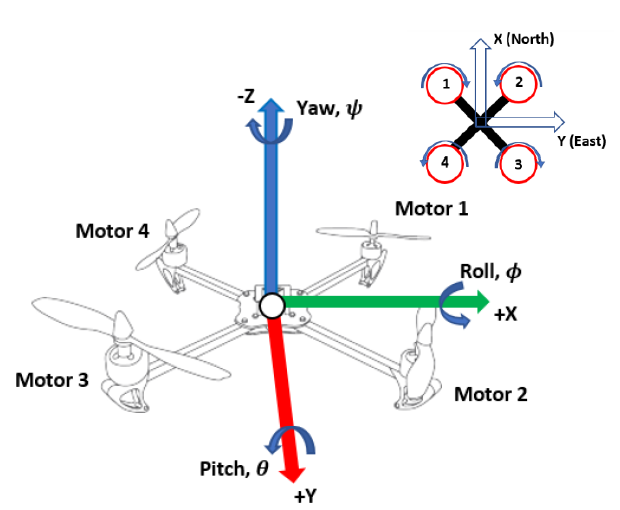
\includegraphics[scale =0.7]{pictures/control/drone directionals.png}
\end{center}
\caption{Quadcopter 'x' configuration \cite{Ferry}}
\end{figure}

The drone's states include critical physical properties like acceleration, velocity, and position, which are all detected by sensors. A gyroscope is used to record the angular changes of the drone. An accelerometer is a device that measures acceleration along the X, Y, and Z axes. Since the gyroscope drifts and the accelerometer has measurement spikes when subjected to high acceleration, a complementary filter will be needed, which will be discussed in the “IMU” subsection. A dedicated infrared sensor is also used to measure distances in the Z-direction, allowing for exact location information.
A state table can be found in Appendix E.

Before plant model equations can be generated, parameters for the drone need to be calculated. The parameters are what explains the drone mathematically and are an integral part of modelling the drone. The more accurate these values are the more realistic the plant model will be.
The parameters needed can be seen in the table below:\cite{Ferry}

\begin{figure}[H]
\begin{center}
    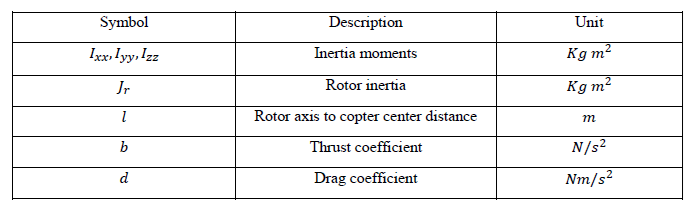
\includegraphics[scale =0.9]{pictures/control/parameter table.png}
\end{center}
\caption{State table}
\end{figure}

\subsubsection{Inertia Moments}
A moment of inertia is a constant value that explains the force/torque required to rotate an object in the direction of the moment. A desired angular velocity around a rotation axis can be found. The moments of inertia are found using estimation. If it is assumed that the drone is symmetrical in all axis, the moments of inertia can be found using parallel axis theorem to approximate the moments for each individual part of the drone in the X, Y, Z directions. For the calculations it’s assumed that the centre of mass for the drone is perfectly in the centre of the drone’s body.
The equations used for each individual part of the drone can be found in \cite{Ferry}.

For the approximation smaller electrical components were not considered, such as wires and mosfets, since their collective total weight is less than a gram, they are deemed negligible for the accuracy estimation.

\begin{figure}[H]
\begin{center}
   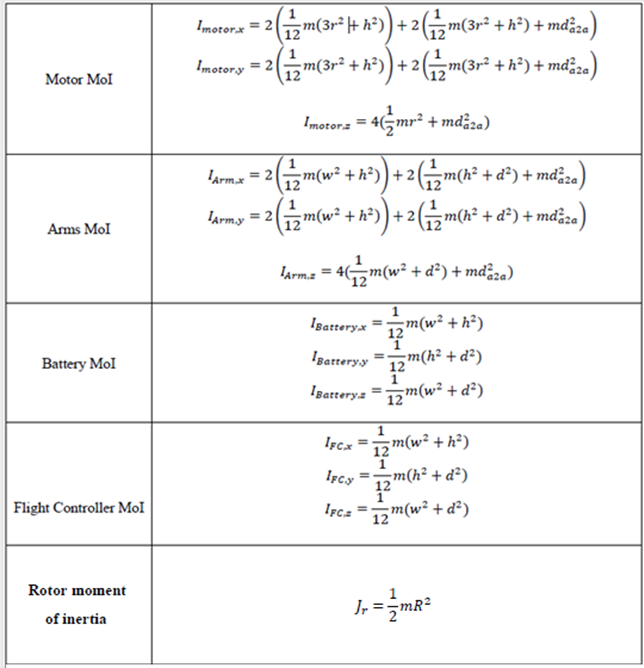
\includegraphics[scale =0.87]{pictures/control/inertia tables table.png}
\end{center}
\caption{Inertia moment equations \cite{Ferry}}
\end{figure}

A mathematical document can be found as a hand-in attachment “SPRO4math”. It shows the detailed process of calculation.
\begin{figure}[H]
\begin{center}
   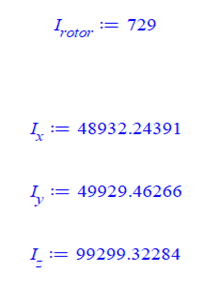
\includegraphics[scale =1]{pictures/control/Inertia moments.png}
\end{center}
\caption{Moments of inertia in the X, Y, Z axis, in $g*mm^2$ as calculated from equations, used in the final version of the quadcopter}
\end{figure}

\subsubsection{Characterization of Motor}
Some drone parameters can not be determined due to a lack of data concerning the motors used in the project. The motors are of a commercial product, but with no available data sheet. This means that motor constants and thrust coefficients need to be determined through testing. 
The next part of the report is a small summary of the tests done to determine the data needed for the motors. The full reports concerning testing and acquiring these values can be found in the appendix. 
\begin{itemize}
    \item Thrust testing can be found in appendix \ref{appendix_thrust}.
    \item Motor constant testing can be found in appendix \ref{Motor Testing_Appendix}.
\end{itemize}

\subsubsection{Thrust testing}

For thrust testing the motor is placed in a frame on a scale to measure the change in weight when the motor is operating. A sketch of the setup can be found in appendix \ref{appendix_thrust}2.2. The motor used had an operating voltage window of 0-4,2 volts, therefore the motor was tested between 1-4,2 volts incremented with 0,1 volts, and the weight change noted for each increment. Characterizing the motor yielded the results seen in figure \ref{fig:motorthrustgraphed}. As a general rule of thumb, provided by project supervisors, the motor's need to produce double the thrust of the total weight of the drone to operate ideally. At maximum voltage level of the battery, a single motor produces 22.2 grams of thrust. In conclusion, at maximum voltage level the drone can ideally weigh 44.4 grams in total. The battery will slowly discharge meaning that it's impossible to always have max output, so it should be a little less than 44.4 grams in practice.

\begin{figure}[H]
\begin{center}
   \includegraphics[scale =1]{pictures/control/Graph thrust.JPG}
   \label{motorthrustgraphed}
\end{center}
\caption{Motor Thrust Graphed}
\end{figure}

\subsubsection{Motor Constants, and Thrust Coefficient}
Motor constants relevant for this project include, “Motor velocity constant” ($K_v$) and “Motor torque constant” ($K_T$)
With a simple setup the motor's RPM can be tested proportionally to PWM. The motor was tested in 20 increments, using a photo sensor to measure RPM. Using the data from the test, we get the result showin in figure \ref{fig:motorconstantscals}. \cite{MotorConstants}

\begin{figure}[H]
\begin{center}
   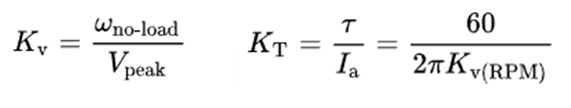
\includegraphics[scale =1]{pictures/control/Motor constants theory.png}
\end{center}
\caption{Equations used for calculating thrust- and velocity constants}
\end{figure}

\begin{figure}[H]
\begin{center}
   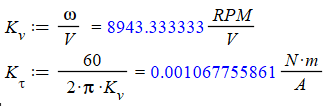
\includegraphics[scale =1.5]{pictures/control/Motor constants calc.png}
   \label{motorconstantscals}
\end{center}
\caption{Motor Constants}
\end{figure}

Combining the two test data sets it is possible to determine the thrust coefficient of the motor. Using the graph from the thrust test, the thrust can be calculated by taking the voltage drop over the motor. This thrust is then divided with the angular velocity to get the thrust coefficient ($TC=3.59E-05$).

The constants/coefficients are calculated around 3.0V inputs, which is the voltage needed to achieve the theoretical hover thrust. This is sensible since most of the time the drone will be operating around these values. 

\subsubsection{Environmental Forces}
The drone is very small, weighing only approximately 60 grams with little surface area. Because of this, aerodynamic effects have been neglected for the modelling. Environmental forces mainly include but are not limited to wind resistance and liftoff turbulence.

\subsubsection{Generating Plant Model Equations}
Now with the all the states and parameters defined, plant model equations can be generated. 
First, we will look at how the motors should operate together to move the quadcopter in the desired direction. A quadcopter can move in X and Y directions using pitch and roll. When the quadcopter rotates around one of its axis, all the rotor blades will generate thrust at an angle, moving the drone in a direction. It is important to control the individual motors so the drone won’t tilt too much, causing it to flip in the air. In figure \ref{fig:ter} below the different cases of directional movement for the quadcopter can be seen.  


\begin{figure}[H]
\begin{center}
   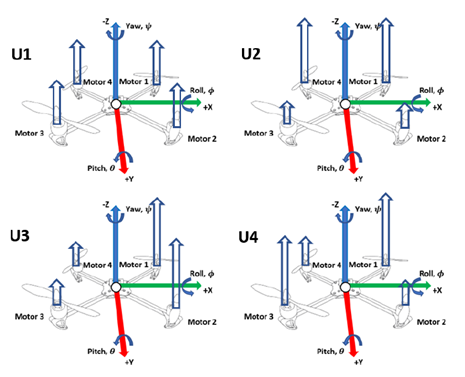
\includegraphics[scale =1]{pictures/control/thrust equations results.png}
   \label{ter}
\end{center}
\caption{Visual representation of thrust equations \cite{Ferry}}
\end{figure}

In figure \ref{fig:ter} U1 is the general thrust behaviour, providing thrust equally and symmetrically to move only the Z axis. U2 creates a roll, thrusting the drone in the Y direction. U3 creates a pitch, thrusting the drone in the X direction. U4 increases the thrust for motors turning the same direction and decreases the thrust of the motors rotating the opposite direction, allowing the drone to rotate in the Z axis e.g., yaw due to non-symmetrical rotational forces created by the moments of the motors.  \cite{Ferry}

Each motor's thrust is then defined as angular rotational speed to acquire the following equations.

\begin{figure}[H]
\begin{center}
   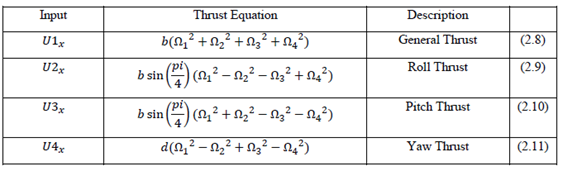
\includegraphics[scale =1]{pictures/control/thrust equations.png}
   
\end{center}
\caption{Thrust equations \cite{Ferry}}
\end{figure}

The plant equations for this project were sourced from \cite{Ferry}. The source has a more in depth description of how the plant equations were found.
A summary of all the plant equations can be found in appendix \ref{appendix_plant}.

\begin{figure}[H]
   \begin{center}
      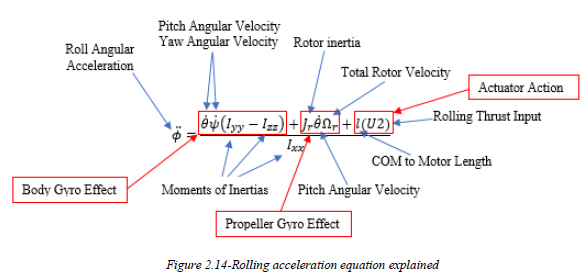
\includegraphics[scale =1]{pictures/control/plant equation example.png}
   \end{center}
   \caption{Example of plant equation for phi. \cite{Ferry}}
   \end{figure}
Body gyroscopic effects from changes in the quadcopter orientation.
Propeller gyroscopic effects from propeller rotation and angle/orientation.
Actuation action forces produced by the rotors/propellers.

\subsubsection{SIMULINK/Matlab Implementation}
To make the Simulink model the thrust equations must be transferred into the program using the angular speed as inputs and the motor parameters. Below the thrust equations can be seen in Simulink with the inputs on the left and outputs on the right. (The outputs are U1, U2, U3, and U4, as well as Omega) In SIMULINK the math is done using “blocks”, the addition and subtraction is performed first, and then the next blocks take the product. Essentially the math is converted using blocks in SIMULINK.

\begin{figure}[H]
\begin{center}
   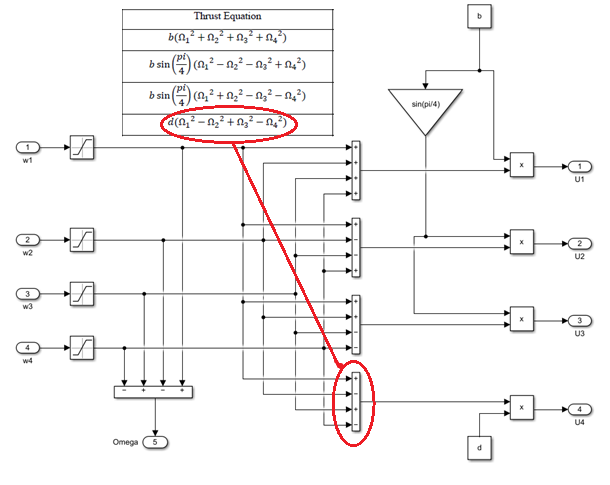
\includegraphics[scale =1]{pictures/control/thrust equation in simulink.png}
\end{center}
\caption{Thrust equations in SIMULINK}
\end{figure}

The rest of the plant equations are then also transferred to SIMULINK using the same process, using blocks to represent the math. The next part of the plant takes the thrust equations as an input to calculate theta, phi, and psi, for position, velocity, and acceleration.

Below is an example for the equation of phi double dot. The thrust equations were used alongside feedback with the drone parameters to get the result. Since all the equations need feedback from the other plant equations, an initial value must be set. It makes sense to make the initial value 0 since it hasen't moved yet and there has been no change in any direction or angle. Throughout the flight the drone will then fill out the theta, phi, and psi values using the sensors to determine the change in position. For example, if the drone is slanted a bit in the direction of motor 4 and 1, the drone will have a change in the roll aka phi value. The sensor will detect the magnitude of this change, and U2 will increase to give more thrust to those motors to stabilize. Thrust is increased proportionally in order smoothen the stabilization. 

\begin{figure}[H]
\begin{center}
   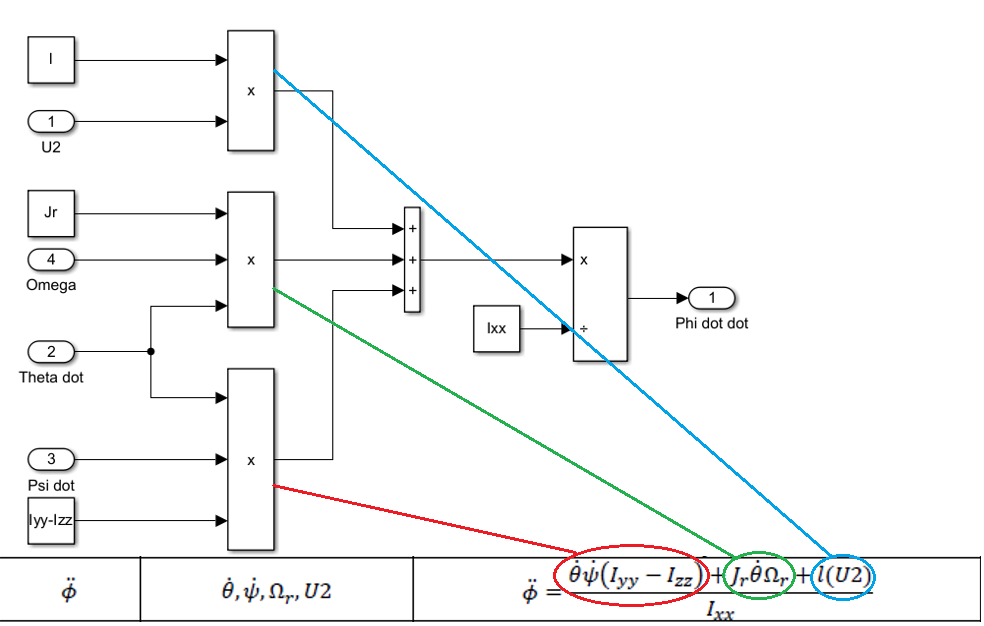
\includegraphics[scale =0.7]{pictures/control/plant equation phi example.png}
\end{center}
\caption{Plant equation for phi double dot}
\end{figure}

\begin{figure}[H]
\begin{center}
   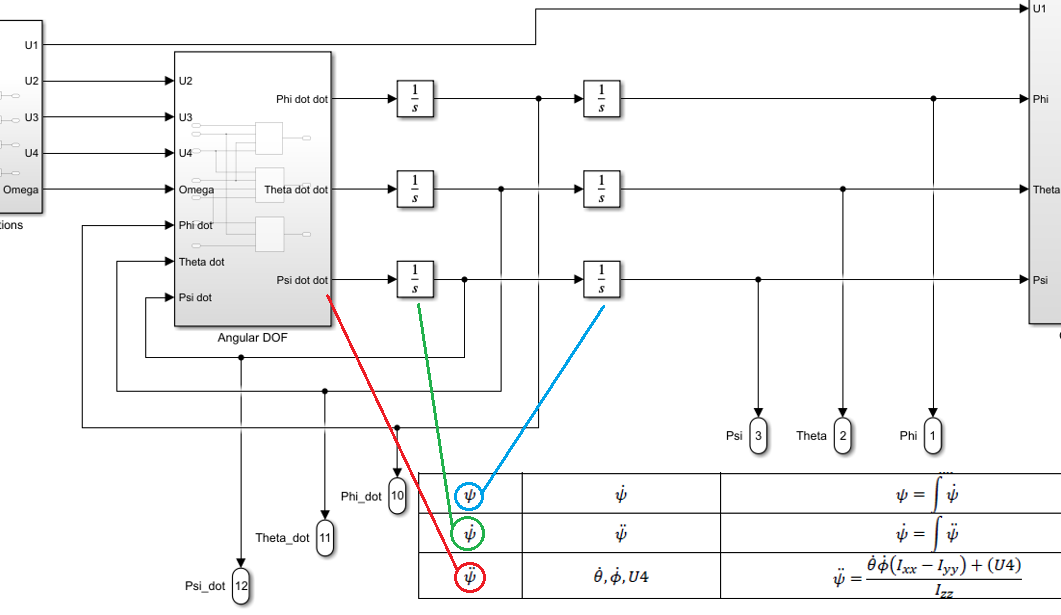
\includegraphics[scale =0.6]{pictures/control/plant pic1.png}
\end{center}
\caption{Angular equations overview example}
\end{figure}

To finish out the plant, the X, Y, and Z values for acceleration, velocity, and position are calculated using the values from theta, phi, and psi, these equations rely on feedback from each other in the same way that angles do, and use the same principles when it comes to determining the initial value. 

\begin{figure}[H]
   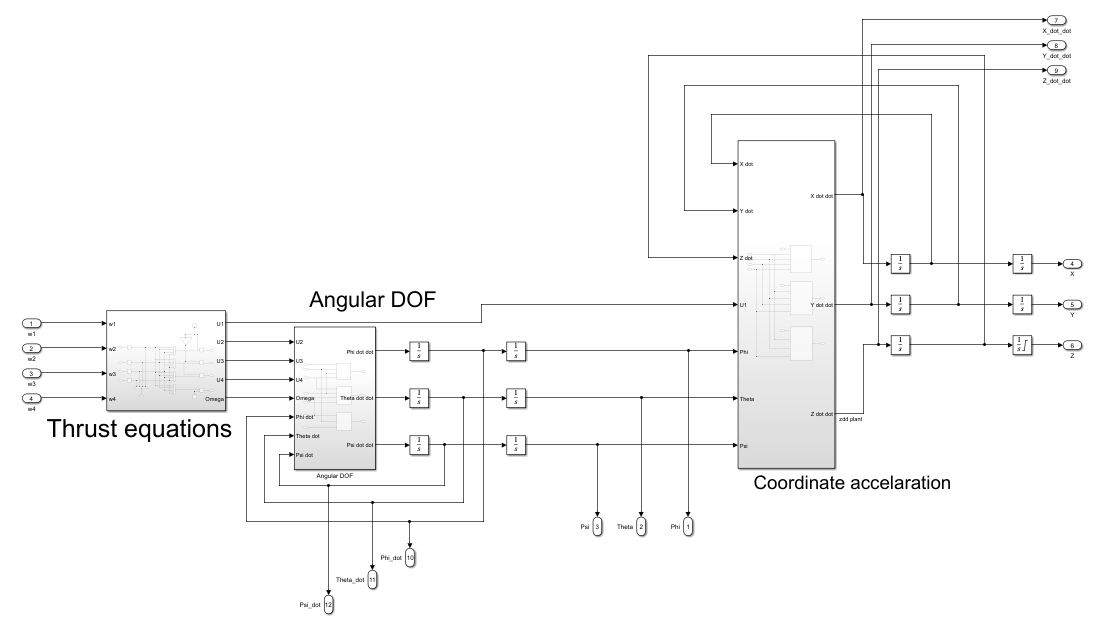
\includegraphics[scale =0.6]{pictures/control/Plant overview.png}
\caption{Plant overview in SIMULINK}
\end{figure}

\section{Software prototyping}
\subsection{Embedded development environment}

Software shoud take care of the motor control, IMU output readings and remote control, this could create complications, as essentially they would interrupt each other. A way of multitasking should be introduced.
"An RTOS (Real-Time Operating System) is a software component that lets you rapidly switch between different running sections of your code. Think of it as having several loop() functions in an Arduino sketch where they all run at the same time." \cite{Joe2019}

After research, the list was narrowed to two top condenders – FreeRTOS and Zephyr. Both solutions are open source, widely used and support the Microcontroller board we have chosen. \cite{Lemberg}
According to 2018 IoT Developer Survey \cite{IOT}, FreeRTOS is one of the most popular OS used and while Zephyr only received a 2.8 \% rating in 2018, it is often described as one of the fastest growing RTOS and in 2022 has become the largest open-source RTOS project by the number of commits and developers. (See Figure~\ref{fig:iot_os})
\begin{figure}[H]
    \centering
    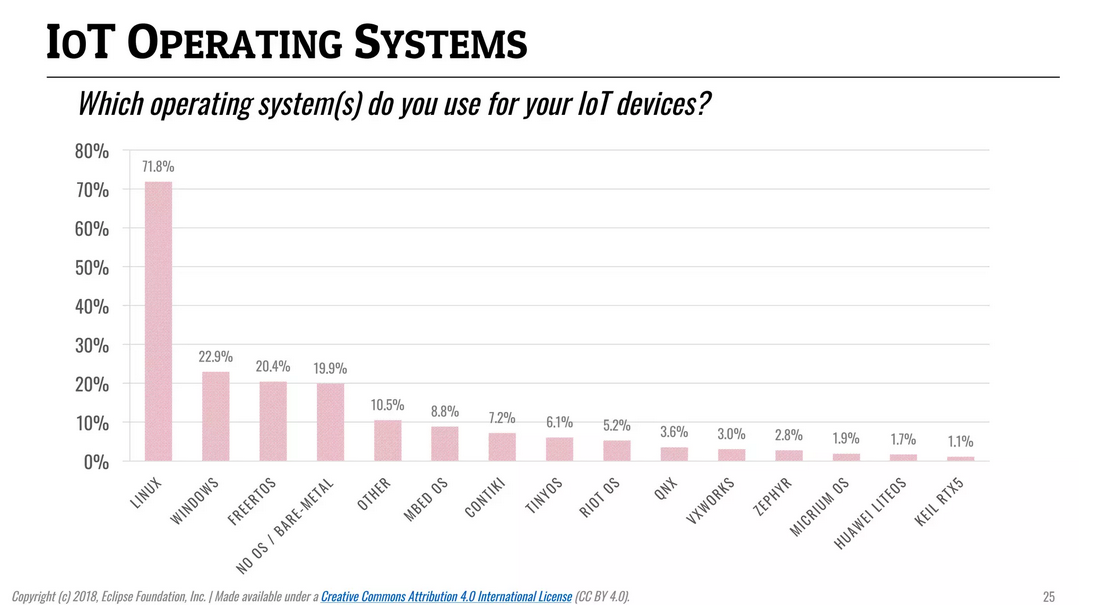
\includegraphics[scale = 0.5]{pictures/iot_os.PNG}
    \caption{IoT Developer Survey 2018 results}
    \label{fig:iot_os}
\end{figure}

To decide between the RTOS choice, a pros and cons table was created and evaluated. \cite{Comparison} (See Table~\ref{table.rtos})

\begin{table}[H]
      \makegapedcells
  \setlist[itemize]{font=\color{black},
                    nosep,
                    leftmargin=*,
                    after=\vspace*{-\baselineskip}}
      \setlength{\tabcolsep}{3pt}
  \begin{tabularx}{\linewidth}{|>{\RaggedRight}p{25mm}|*{2}{I |}}
      \hline
  RTOS
      &   \mcl{Advantages}    &   \mcl{Disadvantages}        \\
      \hline
  FreeRTOS 
      &   \item Suitable for begginers
          \item Open source – online comunity support available 
          \item Libraries for Seeed XIAO Sense available
          \item Constantly improved
          \item Fast code execution
          \item Low memory consuption
          &   \item Not event-driven (scheduler will only be called once in a certain period of time)
              \item Less flexible
              \\
      \hline
  ZephyrRTOS
      &   \item Open source – online comunity support available
          \item Libraries for Seeed XIAO Sense available
          \item Constantly improved
          \item Designed to ensure energy efficiency
          \item Highly configurable
          \item Event-driven
          \item Kernel can create additional system threads
          \item Possible to exclude multithreading
          \item Additional debugging features
          \item Supported by Nordic Semiconductor
          &   \item More difficult to set-up
              \item Potentially complicated to use with no experience
              \\
      \hline

\end{tabularx}
\caption{Comparison between ZephyrRTOS and FreeRTOS}
\label{table.rtos}
\end{table}

It was evaluated, that overall FreeRTOS seems to be a better established more simple solution to be used in case of no experience, whereas Zephyr offers more flexibility and is a fast growing popular solution well suited for our application and would be a worthwile investment to build our skillset for future projects. \cite{Industry}

PlatformIO is an open-source extension of Visual studio code, which supports hundreds of boards with different frameworks. \cite{Platform} Seeed XIAO nRF52840 is not natively suported. Seeed made library for Arduino IDE, which supports Arduino and Mbed framework, that was implemented through Github to PlatformIO and allows non-problematic implementation.
The XIAO has library in the Zephyr Github repository, but the PlatformIO does not use most recent version. The version of Zephyr itself is altered in PlatformIO and therefore does not work even after corssreferencing with other boards already implemented in PlatformIO, such as Seeeduino (as a reference for the formfactor) or nRF52840 DK (as a reference for the chip).
The PlatformIO does not have inbuild serial USB communication, which results in inability to reprogram the board through the VS Code and need to go through bootloader first. This poses inconvinience, which can be avoided by use of a Arduino IDE, therefore if route of MBed or Arduino framework is chosen, Arduino IDE should be chosen. If the route of Zephyr is chosen, SDK by nordic semi is the optimal route, because event though it also does not have serial USB, it uses barebone Zephyr.

Opon further research, the Seeeduino XIAO nRF52840 Sense uses the nRF52840 microcontroler, so looking to Nordic Semiconductor nRF Connect SDK for development, which uses a RTOS called ZephyrRTOS.
Additionally, the SDK provides useful tools for development, such as build, flashing and debugging actions. \cite{nRF}


Seeed XIAO nRF52840 is not natively suported on on nRF Connect SDK, but as ZephyrRTOS supports it. \cite{docsZephyr}

There is a caviat around this, we can fetch profiles from GitHub of the current version of Zephyr via \path{Zephyr/boards/arm/xiao_ble} at main branch \cite{gitZephyr} and import the needed files into the SDK version of Zephyr we have.
In our case the path of the files would be in \path{~\ncs\v2.3.0-rc1\zephyr\boards\arm} .
After doing so, following the steps in the DevAcademy, nRF Connect SDK Fundamentals, Lesson 1 can be followed for setup. Then a blinky application can be created, and built via nRF Connect.
After a build of the application is created, a files for flashing will be created in the "build" subdirectory of the application.
To flash the Seeed XIAO nRF52840 Sense chip, entering a bootloader is needed, as it ships with the Adafruit nRF52 Bootloader, which supports UF2 flashing. \cite{docsZephyr}
Further more, a zephyr.ut2 file can be found in the "build" subdirectory of the application, after building the application, as we have done.
To access the bootloader, connect the Seeed XIAO to a PC.
Now to enter and flash an application, the reset button on the Seeed board should be clicked two times in quick succession, this will propmt the memory of the Seeed board on your PC.
Now find the previously mentioned zephyr.ut2 and drag it in to the memory of the Seeed board, and this will flash the board with the new application.

A issue accured when trying to test the "Hello World" application, when connecting to serial monitor no output is given.
After further investigation, it was noticed that the Seeed documentation, mentiones no debugging interface, hence no USB serial exists.
To solve the issue, an application called "console", from \path{zephyr/samples/subsys/usb/console} was cloned, in order to test a virtual USB serial connection, with the use of CDC ACM UART. \cite{gitZephyr}
After building and flashing, results were achieved. (See Figure~\ref{fig:serial})

\begin{figure}[H]
    \centering
    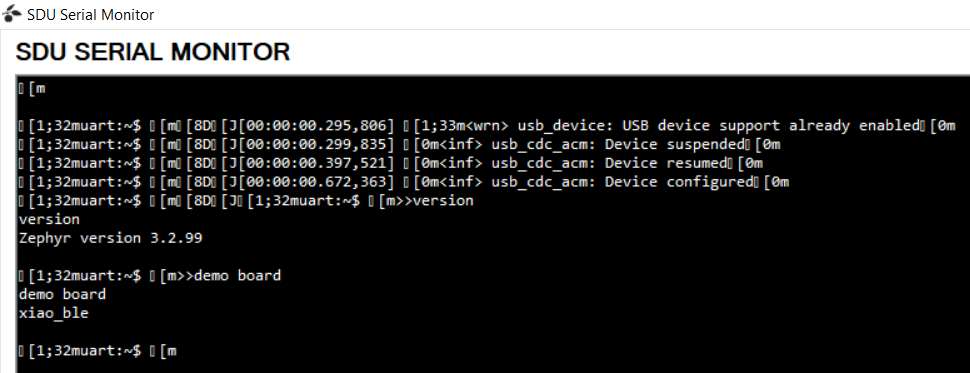
\includegraphics[scale = 0.7]{pictures/serial_monitor.png}
    \caption{Serial output of the XIAO MCU}
    \label{fig:serial}
\end{figure}

Another issue that arose was debugging. The Seeed XIAO nRF52840 Sense does not have any sort of built in debugging tools. \cite{wikiSeeed}
One can use a J-link debugging tool, but a caviet was found, which was GDB stub, which Zephyr supports, this would save budget. \cite{docsZephyr}

After achieving a succesful development cycle, it was conducted, that the use of ZephyrRTOS is possible with our current setup.
After further consultation with the supervisors, it was conducted, that the writers of the project have no skills in RTOS, more specifically in threading, and with the guidence of Davi, it was concluded, that acquiring such skills would be outside the scope of the project, as the main focus is control engineering.
\subsection{QuickPID}
For implementing the PID controller on the MCU, the QuickPID library was chosen. QuickPID is an updated implementation of the Arduino PID library with additional features for PID control. \cite{QuickPID} It was chosen due to the following reasons:
\begin{itemize}
    \item
        Advanced Anti-Windup Mode: When compared to the normal PID implementation, the library features a more robust anti-windup mode. Integral windup can occur when the controller's integral term accumulates error during periods of saturation or when the actuator cannot keep up with the needed control effort, and anti-windup approaches help prevent this. \cite{QuickPID} The QuickPID library can lessen integral windup, reduce overshoot, and improve stability during transient situations by adding an advanced anti-windup mode.
    \item
    	Timer-Based Control: QuickPID is a timer-based control option that lets you use external timers or Interrupt Service Routines (ISRs) for precise timing control. \cite{QuickPID} This functionality is especially beneficial in systems with strict timing requirements or when employing external devices or sensors that are synced with the control loop. In this situation, if issues with the IMU or the controller develop, the timer-based technique can simply remedy them.
    \item
    	Compatibility with Arduino IDE: updated implementation of the Arduino PID library. As the Arduino ecosystem was chosen over Zephyr RTOS using the QuickPID library provides a seamless integration.
\end{itemize}
When utilizing the library, the PID compute sample time, default = 100000 µs, was changed to 2500 µs to match the IMU 400 Hz measuring frequency. Matching the PID sample frequency with the IMU measuring frequency ensures synchronization, consistent data availability, and accurate control in quadrotor systems. It enables the PID controller to operate based on up-to-date sensor measurements, respond effectively to dynamic changes, simplify system identification and tuning, and optimize computational efficiency. Additionally, the output limits of the PID (0-255 by default), were changed to (-255) – (255), as a negative error can be achieved in the quadrotor system.

\subsection{NanoBLEFlashPrefs}
Data logging has evolved as a significant approach for overcoming the issues of the PID tuning process. \cite{PIDlog}
During quadrotor operation, data logging entails recording numerous flying characteristics, sensor measurements, control inputs, and system responses.
Engineers and researchers can obtain useful insights into the quadrotor's behavior and make informed judgments to fine-tune PID controller parameters by collecting this comprehensive set of data. \cite{loggingProof}
Data logging also allows for the comparison and evaluation of various PID tuning strategies or algorithms. 
Thru analysis, the influence of each adjustment on the system's behavior by methodically changing PID controller parameters can be observed in the quadrotor's response.
This iterative method makes it easier to identify ideal PID parameter combinations that produce the required flight characteristics.
The Seeduino XIAO nRF52840 lacks an inbuilt EEPROM (Electrically Erasable Programmable Read-Only Memory). The nRF52840 SoC has 1 MB of inbuilt Flash memory, and the XIAO board has 2MB of onboard flash memory for storing data. The choice was based on the following benefits of adopting flash memory:
\begin{itemize}
    \item
        Faster Read and Write Operations: Flash memory generally offers faster read and write speeds compared to EEPROM.\cite{Sandeep} This will be advantageous in the iteration process when there is a need to access data quickly or update it frequently.
    \item
    	Endurance and Lifetime: Flash memory typically has a higher endurance level than EEPROM. It can withstand a larger number of read and write cycles before it starts to degrade.\cite{Sandeep} This endurance is particularly important when you need to update or modify the contents of the memory frequently.
    \item
    	Cost and Space Efficiency: Since the nRF52840 chip already integrates Flash memory, using it eliminates the need for an additional EEPROM chip. This reduces the component count, simplifies the PCB layout, and potentially lowers the overall cost and space requirements of your design.
\end{itemize}
NanoBLEFlashPrefs is a Arduino library, which is a substitute for missing EEPROM storage on Arduino Nano 33 BLE and 33 BLE Sense (not for Nano 33 IoT or other Nano boards). \cite{FlashPrefs}
As the Seeduino XIAO nRF52840 Sense uses the same SoC chip as the Arduino Nano 33 BLE Sense, it can be easily used for the project. \cite{Nano33} \cite{wikiSeeed}
Unfortunately, the library requires Mbed OS; nonetheless, due to its design principles and development architecture, it is frequently regarded as easier to use than other Real-Time Operating Systems (RTOS). Furthermore, it is tightly integrated with the Arduino IDE,\cite{MbedNano}, which is utilized as the IDE of choice for writing code to the quadrotor. Because it supports filesystems and storage APIs, Mbed OS is necessary. Mbed OS features lightweight filesystems like FAT and LittleFS that make it easier to read, write, and manage data on flash memory. \cite{MbedWiki}
These filesystems abstract away the complexity of direct flash memory access, allowing for more ordered data storage and retrieval. Furthermore, because Mbed is a simple RTOS, it can be easily adopted for Bluetooth logging, which could be necessary in the future. As it does not have memory constraints, but would be limited in processing power, allowing an additional thread to be used.

\bibliographystyle{plain}
\bibliography{references}
\appendix
\section{Motor Thrust Testing}\label{appendix_thrust}
The 4th semester project in mechatronics is based on building a VTOL drone. For the drone to take flight, 
sufficient thrust provided by the propellers attached to the motors of the drone is required. Thus,
the following is the report of thrust testing using different motors and propellers.
Initial testing setup

\subsection{Initial Assumptions}
The initial idea to test the thrust provided by a certain motor was to create a x-shaped frame where, 
the motors were connected to their respective corners and a bolt was tightened in the centre as a means of weight. 
The frame with the motors were then placed on a scale where the motors were facing in the direction of the ceiling, 
thus meaning that propellers were pushing the air downwards and the setup upwards. The initial weight of the frame was then noted, 
where after powering up the motors, the weight of the setup would decrease due to the thrust. 

\subsection{Initial Results}
The setup of the bolt supporting the frame on the scale was unstable, and because of that the wiring of the motors had also
interfered with the weight. Additionally, as the propellers were pushing the frame with a certain thrust force, 
the air that was being pushed down also had the same force. Therefore, as the frame was very close to the scale, 
the force by which the setup was being lifted by was also being pushed down by the air on the scale, thus making almost no 
changes on the scale readings. 

\begin{figure}
    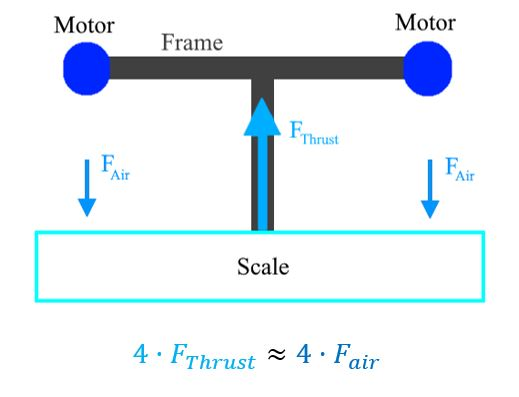
\includegraphics[width=\linewidth]{pictures/control/Motor thrust 1.jpg}
    \caption{Initial Thrust Setup}
    \label{fig:Initial Thrust Setup}

\end{figure}

\subsubsection{Final Assumptions}
To fix the problems of the initial test setup, a second version of the x-shaped frame was made where the corners were connected to 3d printed pillars, 
to make the system more stable. Additionally, instead of placing all the motors at each corner and measuring thrust, only one motor would be placed in the centre instead, 
as the other motors were identical and thus would produce close to identical thrust. Moreover, the motors would now be placed in a direction opposite to the ceiling as then the air would not be pushed on the scale, 
but the frame would be. Thus, the additional weight that occurs after the motors are powered on would be equal to the thrust provided by the motor and propeller.

\begin{figure}
    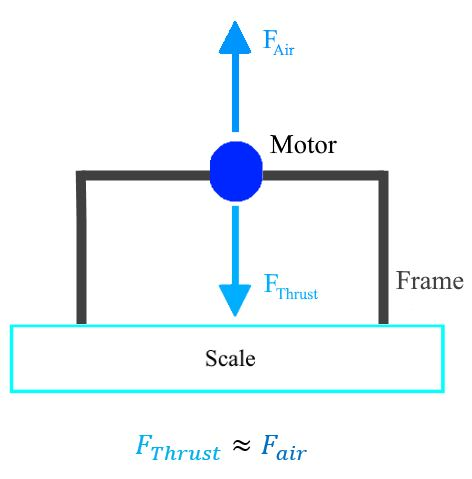
\includegraphics[width=\linewidth]{pictures/control/Motor thrust 2.jpg}
    \caption{Final Thrust Setup}
    \label{fig:Final Thrust Setup}

\end{figure}

\subsubsection{Final Results}

The motor used had an operating voltage window of 0-4,2 volts, therefore the motor was tested between 1-4,2 volts incremented with 0,1 volts. 
Characterizing the motor yielded the following results:

\begin{figure}
    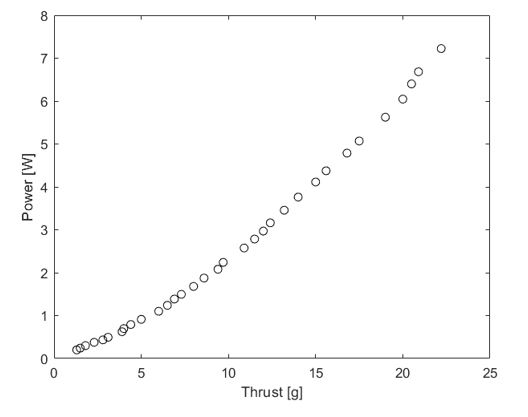
\includegraphics[width=\linewidth]{pictures/control/Graph Thrust.jpg}
    \caption{Motor Thrust Graphed}
    \label{fig:Final Thrust Setup}

\end{figure}

It became clear that the total thrust that could be produced by a single motor was 17.5 grams at 3.7 Volts 
(The minimum level of the battery). Subtracting the weight of the motor itself, the motor can produce a net thrust of 12.4 grams, 
and since the drone would be flown in a quad configuration, the total net thrust possible for the four motors were 49.6 grams at lowest voltage. 
This then set the limits of how heavy the drone could be, and since a general rule of thumb is that the motors need to produce double the needed thrust to lift the drone , 
it’s clear that the remaining components of the drone can weigh 24,8 grams for it to handle optimally. At maximum voltage level of the battery, a motor produces 22.2 grams of thrust, 
so an excess of 17,1 grams subtracting the motors weight itself. So at maximum voltage level, the drones remaining components can weigh 34.2 grams.  

\end{document}
